\documentclass[10pt]{article}
\usepackage[margin=0.72in]{geometry}
\usepackage{booktabs}
\usepackage{graphicx}
\usepackage{microtype}
\usepackage{xcolor}
\title{Persistent Update-Only Evaluation Across Real Graphs}
\author{}
\date{July 31, 2026}
\begin{document}
\maketitle

\paragraph{Question and protocol.}
This experiment asks whether Spine has an update-throughput advantage when
graph computation is disabled (the equivalent of \texttt{max\_iter=0}).  Both
architectures retain graph state across batches.  Spine receives only the
initial graph and each arriving batch.  The official-style GraSU baseline is
future-aware: it receives the complete update trace, performs update-density
reordering once, and reserves PMA slots for that trace.  We therefore report
two distinct metrics: (1) accelerator device cycles for structure updates only,
and (2) finite-trace time including measured CPU preprocessing plus a common
parameterized 12 GB/s H2D and 10 $\mu$s launch/synchronization cost per batch.
No SSSP, PageRank, CC, convergence loop, or ReGraph compute stage runs.

All admitted rows pass every per-batch and final graph-state check.  The primary
cross-dataset experiment uses ten persistent insertion batches of 4,096 records
each.  Host timing is the median of three runs on AU, SU, and WK; memory-heavy SO
and PK use one exploratory host run and are marked as such in the evidence.

\begin{figure}[h]
  \centering
  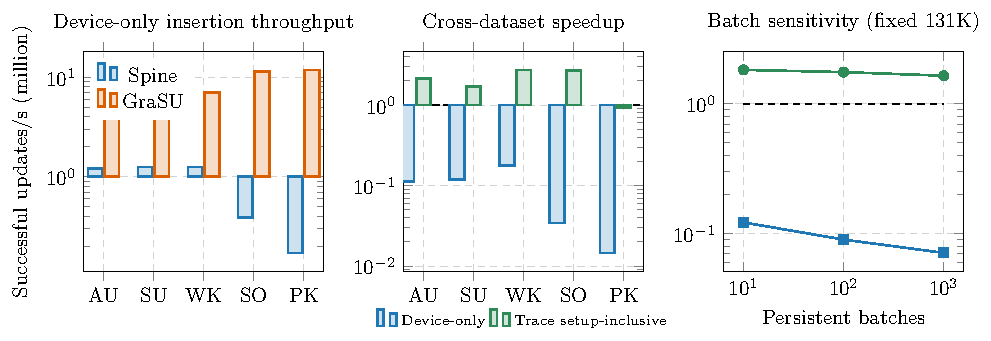
\includegraphics[width=\linewidth]{../figures/persistent_update_campaign_20260731.pdf}
  \caption{Persistent update-only results. Left: pure device insertion
  throughput. Center: Spine/GraSU speedup for device-only and finite-trace
  setup-inclusive time; values above one favor Spine. Right: the same 131,072
  AU records split into 10, 100, and 1,000 persistent batches, isolating
  per-batch overhead rather than trace-length amortization.}
\end{figure}

\begin{table}[h]
\centering
\small
\begin{tabular}{lrrrrrr}
\toprule
Graph & Vertices & Initial edges & Spine & GraSU & Device & Setup incl.\\
 & & & Mupd/s & Mupd/s & speedup & speedup\\
\midrule
AU & 515,281 & 390,847 & 1.215 & 10.845 & 0.112$\times$ & 2.143$\times$\\
SU & 567,316 & 616,118 & 1.248 & 10.484 & 0.119$\times$ & 1.704$\times$\\
WK & 1,140,149 & 1,142,352 & 1.251 & 6.982 & 0.179$\times$ & 2.744$\times$\\
SO & 6,024,271 & 23,724,166 & 0.391 & 11.364 & 0.034$\times$ & 2.683$\times$\\
PK & 1,632,803 & 44,603,928 & 0.172 & 11.815 & 0.015$\times$ & 0.927$\times$\\
\bottomrule
\end{tabular}
\caption{Insertion results for 40,960 successful updates in ten batches.}
\end{table}

\paragraph{Result.}
GraSU's PMA device path is faster on every graph, by 5.6$\times$--68.6$\times$.
The performance gap widens on SO and PK because Spine issues substantially more
backend requests (171,943 vs. 21,779 on SO and 529,909 vs. 16,571 on PK).  Thus
the current evidence does \emph{not} support a Spine update-kernel-throughput
claim.  For a short ten-batch known trace, including preprocessing reverses the
ranking on AU, SU, WK, and SO because GraSU pays its one-time reorder/PMA-build
cost; PK is already an exception, with GraSU about 1.08$\times$ faster even
under that setup-inclusive metric.  Setup-inclusive results are finite-trace
amortization results, not device-throughput results.

\paragraph{Batch and operation sensitivity.}
With a fixed 131,072-record AU trace, increasing the batch count from 10 to
1,000 reduces Spine's device speedup from 0.122$\times$ to 0.071$\times$ and
its setup-inclusive speedup from 1.830$\times$ to 1.650$\times$.  More launch
boundaries hurt Spine; this sweep must not be interpreted as increasing trace
length.  On AU, deletion gives 1.472 Mupd/s for Spine and 9.903 Mupd/s for
GraSU, close to the insertion result (1.385 vs. 10.278 Mupd/s).  Weight
increases are excluded: the frozen Spine differential merge retains the
minimum weight, so that operation requires the separately evaluated full-graph
fallback rather than this pure update-only path.

\paragraph{Scope.}
The simulator uses the common SST memHierarchy/DRAMSim3 backend and finite
FIFO/AXI paths.  The 12 GB/s transfer and 10 $\mu$s launch terms are shared
parameters, not measured XRT timings.  The Bitcoin full graph is excluded by
architecture capacity (24,575,382 vertices exceeds Spine's frozen
$2^{24}$-vertex bound), not by timeout.  Future-unknown online GraSU rebalancing
is a separate baseline and is not silently substituted here.

\end{document}
